
\section{Kernel smoothing methods}
\subsection{One-dimensional kernel smoothers}
We have seen the \textit{k-nearest neighbourhood} average as an estimate of the regression function $\E(Y|X=x)$:
\begin{equation}
\hat{f} = Ave(y_i|x_i\in N_k(x))
\end{equation}
where $N_k(x)$ is the set of $k-points$ nearest to $x$ in squared distance. An example of the resulting fitting curve is shown in green on the left of \autoref{nearest}. The green curve is bumpy, since $\hat{f}(x)$ is discontinuous in $x$. As we move $x_0$ from left to right, the k-nearest neighbourhood remains constant, until a point $x_i$ to the right of $x_0$ becomes closer than the furthest point $x_{i'}$ in the neighbourhood to the left of $x_0$, at which time $x_i$ replaces $x_{i'}$. 
\begin{figure}
\centering
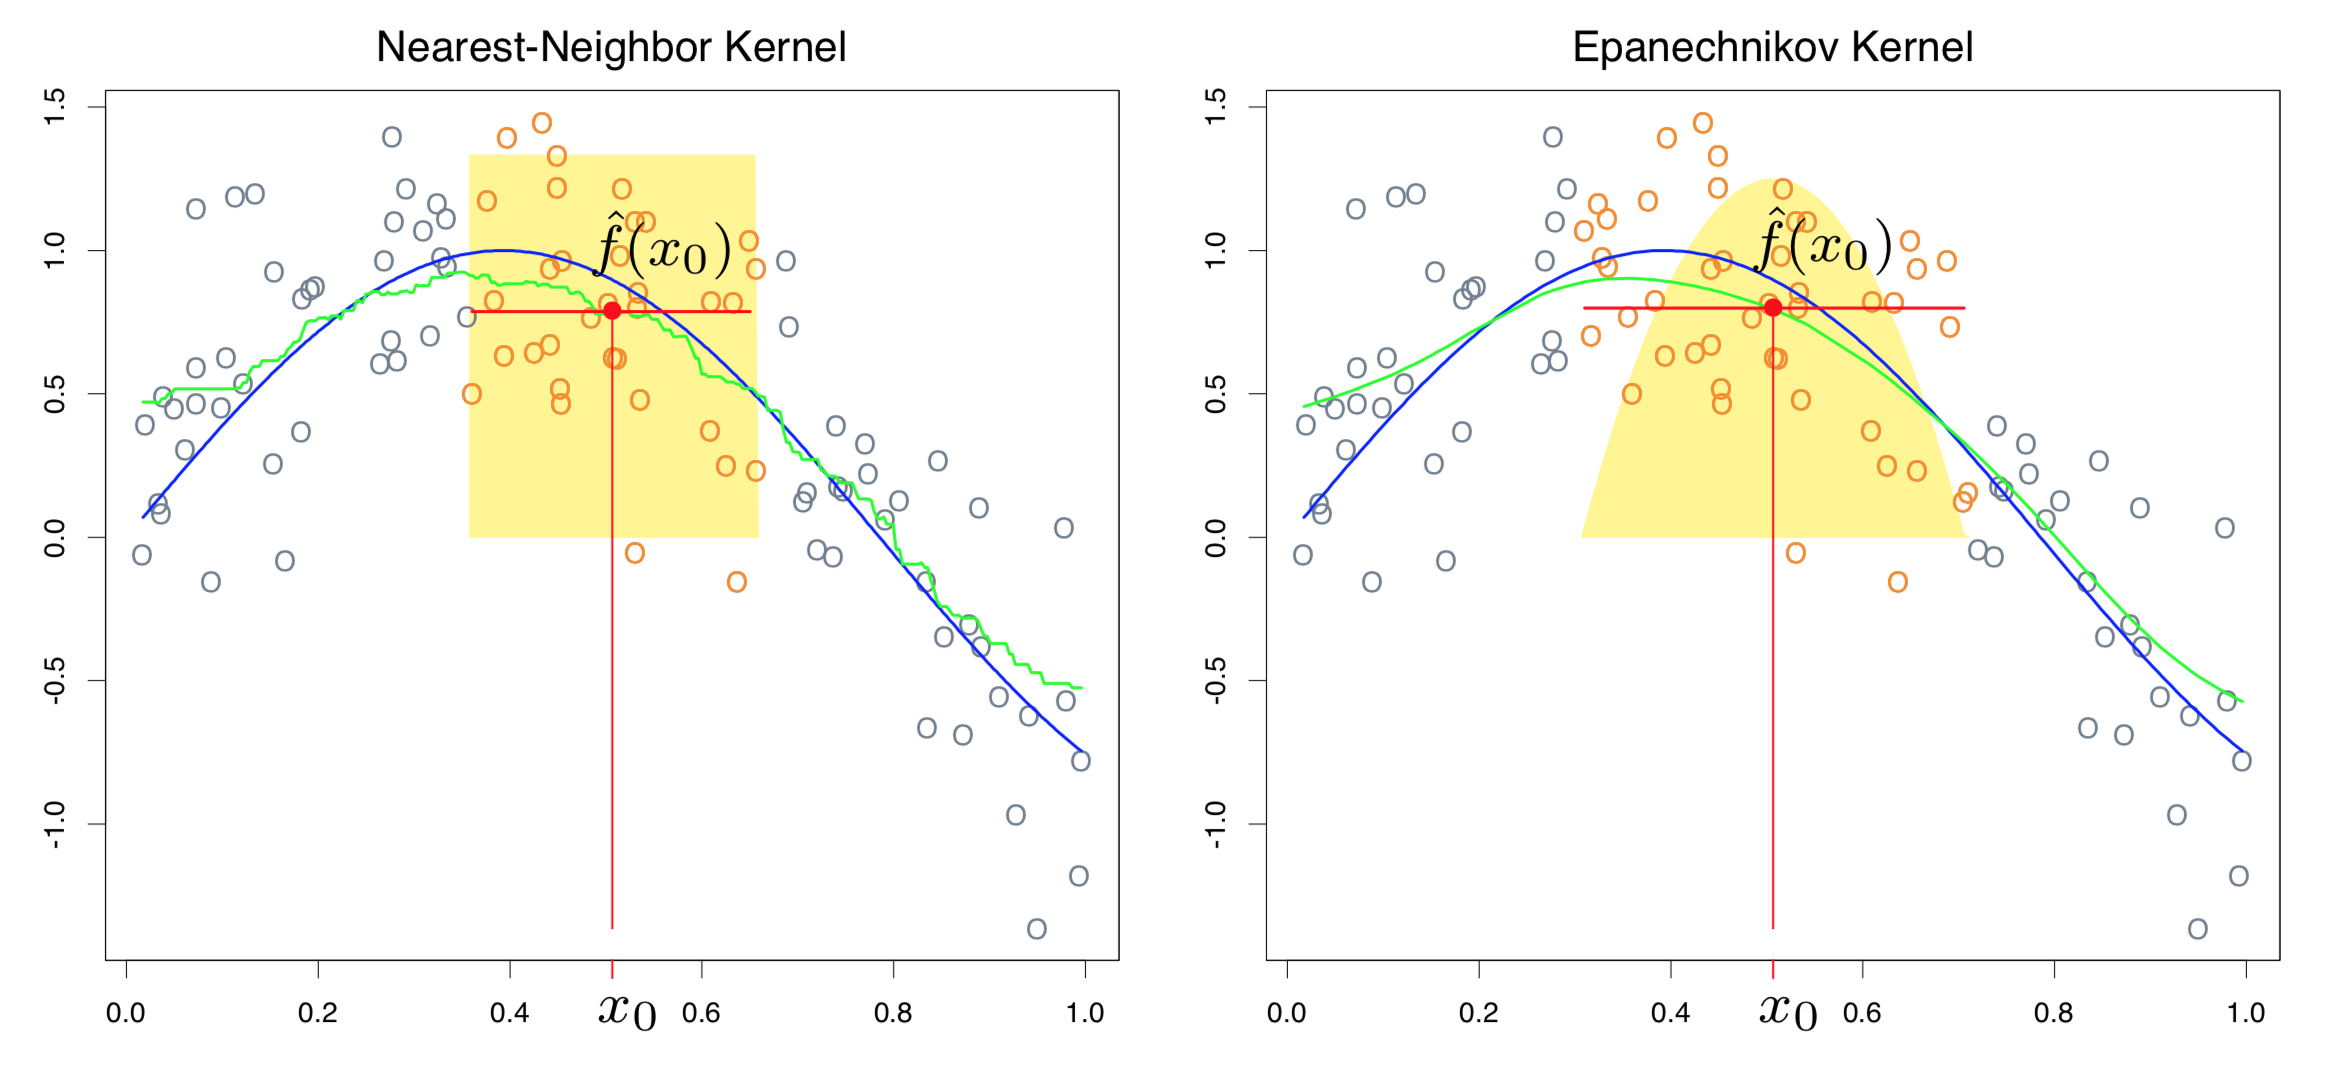
\includegraphics[scale=0.38]{img/nearest}
\caption{In green the fitting curves. On the left the one resulting from \textit{k-nearest neighbourhood}, on the right the metric neighbourhood.}
\label{nearest}
\end{figure}

Rather than give all the points in the neighbourhood equal weights, we can assign weights that die off smoothly with distance from the target point. The right panel in \autoref{nearest} shows an example of this, using the so-called Nadaraya–Watson kernel-weighted average:
\begin{equation}
\hat{f}(x) = \frac{K_\lambda(x_0, x_i)y_i}{\sum_{i=1}^N K_\lambda(x_0, x_i)}
\end{equation}
with the Epanechnikov quadratic kernel:
\begin{equation}
K_\lambda(x_0, x_i)= D\br{\frac{|x-x_0|}{\lambda}} = \left\{ \begin{array}{ll}  \frac{3}{4}\left[1-\left(\frac{|x-x_0|}{\lambda} \right)^2 \right]&\quad if \frac{|x-x_0|}{\lambda}\le 1\\
0 &\quad otherwise
\end{array}
 \right.
\end{equation}
Now the function is continuous. As we move the target from left to right, points enter the neighbourhood initially with weight zero, and then their contribution slowly increases. Note that $\lambda$ dictates the width of the window which is fixed. On the contrary, for the \textit{k-nearest neighbourhood} the window size depends on the density since anyway $k$ points must be considered. \autoref{kernels} shows other kernels. Another popular one is the tri-cube function:

\begin{equation}
 D\br{\frac{|x-x_0|}{\lambda}} = \left\{ \begin{array}{ll}  \left[1-\left(\frac{|x-x_0|}{\lambda} \right)^3 \right]^3&\quad if \frac{|x-x_0|}{\lambda}\le 1\\
0 &\quad otherwise
\end{array}
 \right.
\end{equation}

Both are compact functions. A common non-compact function is the Gaussian function.

Generalizing we can use a width function $h_\lambda(x_0)$ that determines the width of the neighbourhood at $x_0$ (previously we have used $h_\lambda(x_0) = \lambda$.

\begin{figure}
\centering
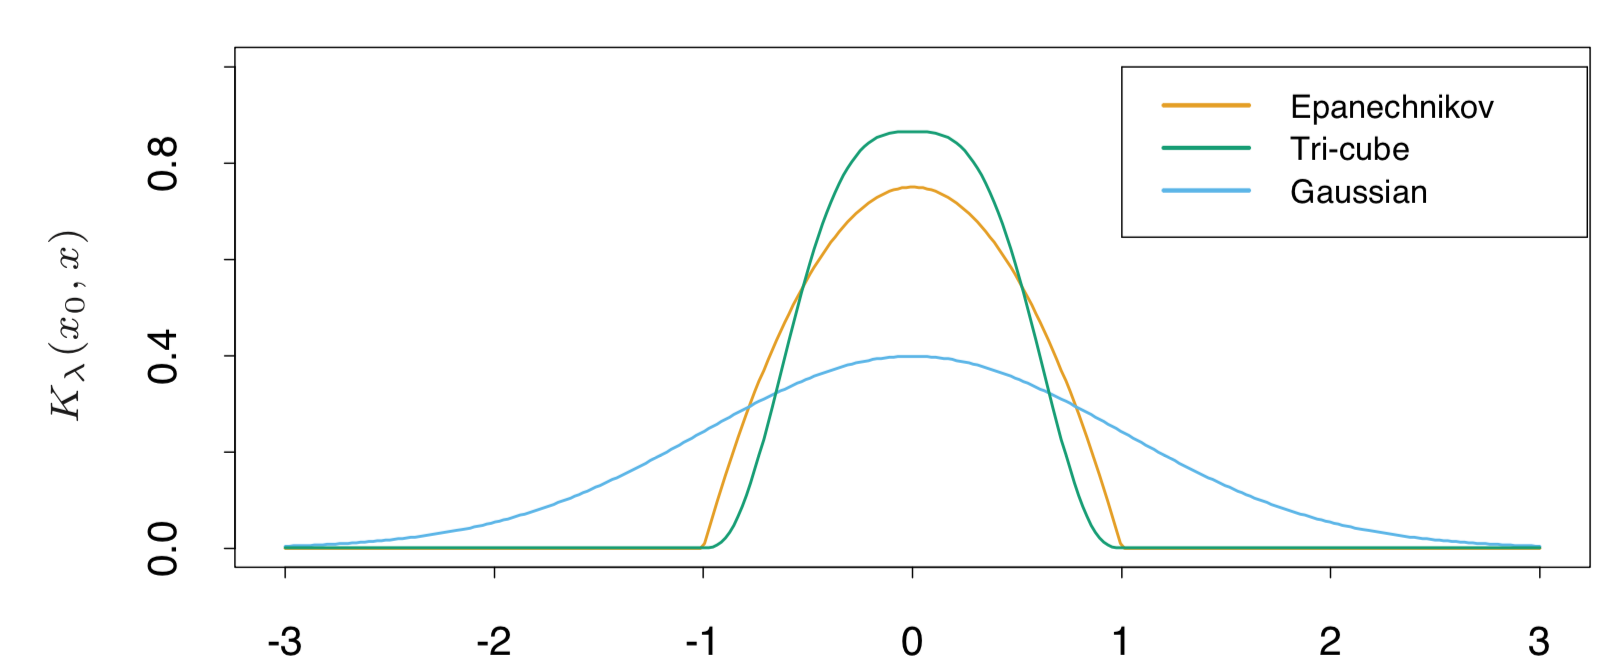
\includegraphics[scale=0.4]{img/kernels}
\caption{A comparison of three popular kernels for local smoothing. Each has been calibrated to integrate to 1. The tri-cube kernel is compact and has two continuous derivatives at the boundary of its support, while the Epanechnikov kernel has none. The Gaussian kernel is continuously differentiable, but has infinite support.}
\label{kernels}
\end{figure}

There are a number of details to be clarified:
\begin{itemize}
\item the value of $\lambda$ which selects the window size. Large values imply lower variance but higher bias;
\item $h_\lambda(x_0)$ can be constant (i.e., $h_\lambda(x_0)=\lambda$) or variable. Constant values (\textbf{metric window widths} keep the bias constant but the variance is inversely proportional to the local density. Nearest neighbourhood has opposite behaviour: the variance stays constant and the absolute bias varies inversely with local density.
\item boundary issues: the metric neighbourhood tend to contain less points on the boundaries while the nearest-neighbourhood get wider.
\end{itemize}

\subsubsection{Local linear regression}
Smooth kernel fit still has a problem close to the boundaries: because of the asymmetry in this region weighted averages can be badly biased (left in \autoref{biasedKernel}). By fitting straight lines rather than constants locally, we can remove this bias effect. Actually, this bias can be present in the interior of the domain as well, if the $X$ values are not equally spaced.
\begin{figure}
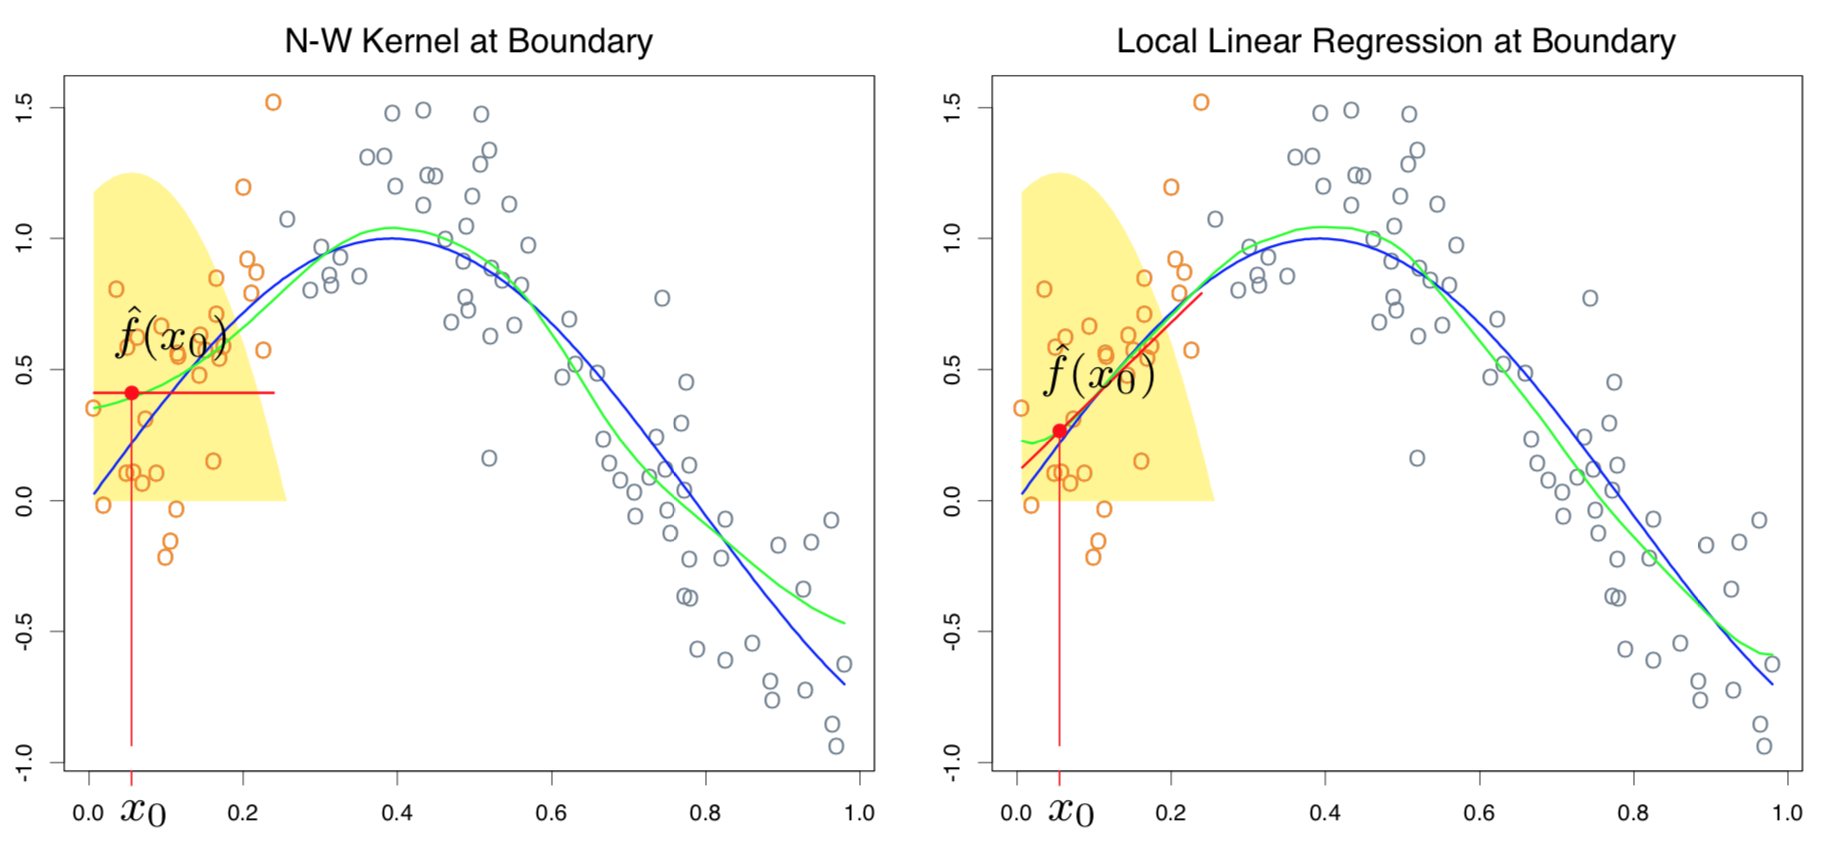
\includegraphics[scale=0.4]{img/biasedKernel}
\caption{On the left it can be noticed the bias effect at the boundaries.}
\label{biasedKernel}
\end{figure}
Locally weighted regression solves a separate weighted least squares problem at each target point $x_0$:
\begin{equation}
min_{\alpha(x_0), \beta(x_0)} \sum_{i=1}^N K_\lambda(x_0,x_1)\left[ y_i - \alpha(x_0) -\beta(x_0)x_i\right]^2
\end{equation}
and the estimate becomes:
\begin{equation}
\hat{f}(x_0) = \hat{\alpha}(x_0) + \hat{\beta}(x_0) x_0
\end{equation}
Notice that although we fit an entire linear model to the data in the region, we only use it to evaluate the fit at the single point $x_0$.

Define the vector-valued function $b(x)^T = (1, x)$. Let $B$ be the $N \times 2$ regression matrix with i-th row $b(x_i)^T$ , and $W(x_0)$ the $N \times N$ diagonal matrix with $i-th$ diagonal element $K_\lambda(x_0,x_i)$. Then
\begin{equation}
\hat{f}(x_0)= b(x_0)^T(\mathbf{B}^T\mathbf{W}(x_0)\mathbf{B})^{-1} \mathbf{B}^T\mathbf{W}(x_0)\y= \sum_{i=1}^N l_i(x_0)y_i
\end{equation}
The weights $l_i(x_0)$ combine the weighting kernel $K_\lambda(x_0, \cdot)$ and the least squares operations and are referred to as the equivalent kernel.Local linear regression automatically modifies the kernel to correct the bias exactly to
first order, a phenomenon dubbed as \textbf{automatic kernel carpentry}.

\subsubsection{Local polynomial regression}
We can fit local polynomial fits of any degree $d$:
\begin{equation}
\begin{aligned}
&min_{\alpha(x_0),\beta_j(x_0),j=1,\cdots,d} \sum_{i=1}^N K_\lambda(x_0,x_i)\left[ y_i - \alpha_0 -\sum_{j=1}^d\beta_j(x_0)x_i^j\right]^2\\
&\hat{f} = \hat{\alpha}(x_0) + \sum_{j=1}^d \hat{\beta}_j(x_0)x_0^j
\end{aligned}
\end{equation}
Local linear fits tend to be biased in regions of curvature of the true function, a phenomenon referred to as \textbf{trimming the hills} and \textbf{filling the valleys}. Local quadratic regression is generally able to correct this bias. There is of course a price to be paid for this bias reduction, and that is increased variance. The fit in the right panel of \autoref{localLinQuad} is slightly more
wiggly, especially in the tails.
\begin{figure}
\centering
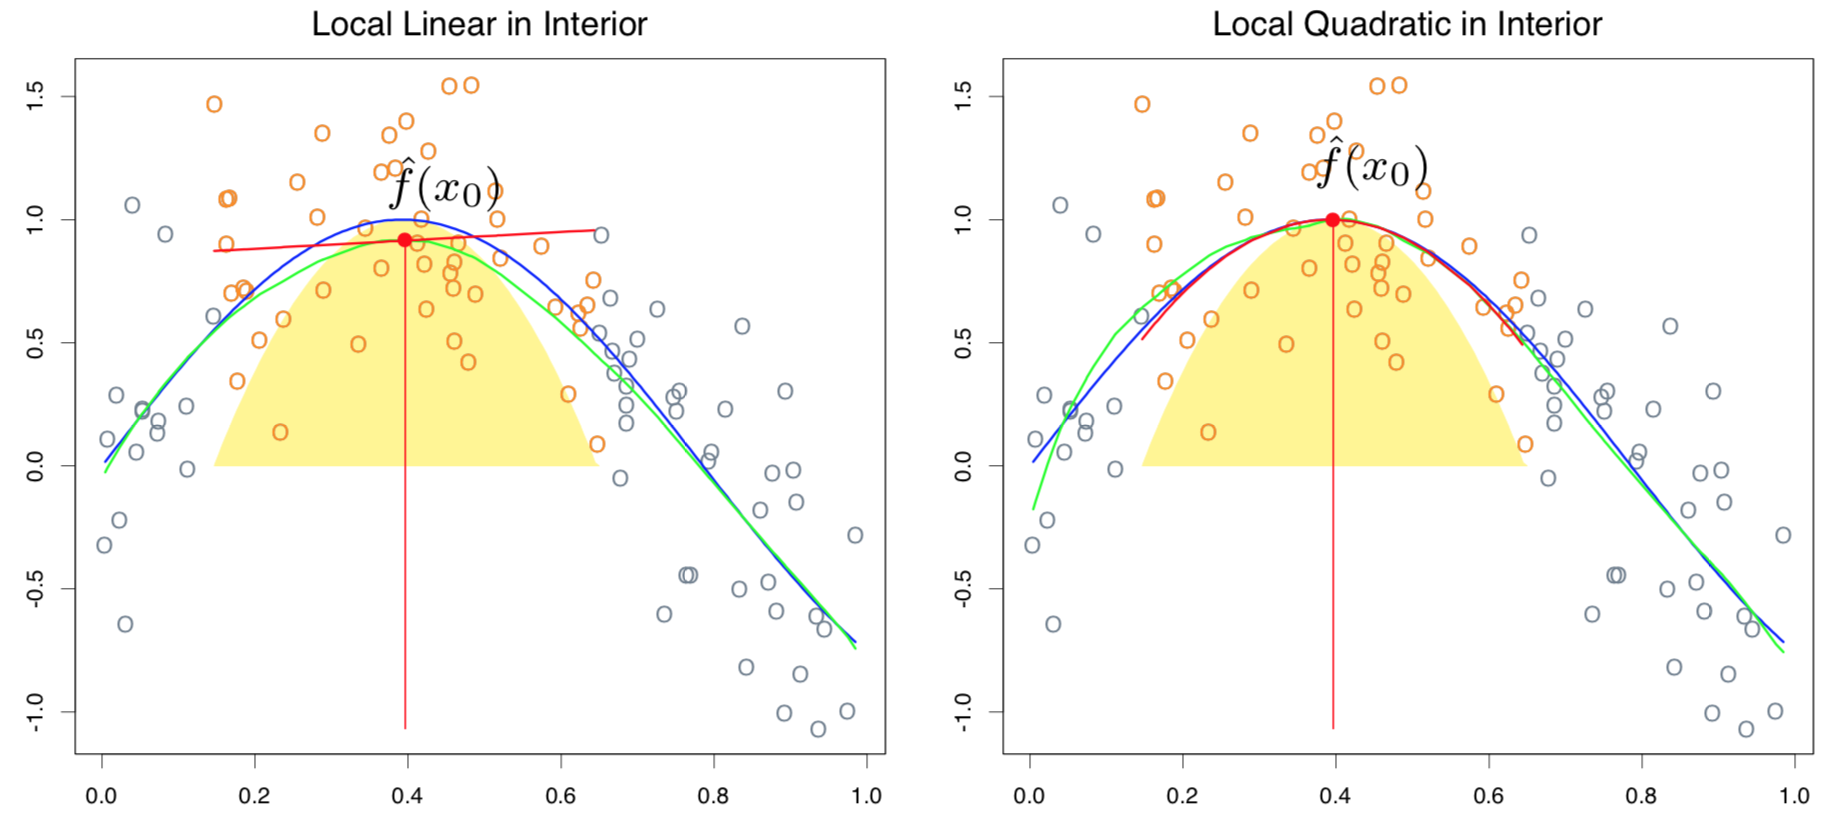
\includegraphics[scale=0.4]{img/localLinQuad}
\caption{Local linear fits exhibit bias in regions of curvature of the true function. Local quadratic fits tend to eliminate this bias.}
\label{localLinQuad}
\end{figure}
Summarizing, local linear fits can help bias dramatically at the boundaries at a modest cost in variance. Local quadratic fits do little at the boundaries for bias, but increase the variance a lot. Local quadratic fits tend to be most helpful in reducing bias due to curvature in the interior of the domain. Asymptotic analysis suggest that local polynomials of odd degree dominate those of even degree. This is largely due to the fact that asymptotically the MSE is dominated by boundary effects.
\subsection{Local regression in $\CMcal{R}^p$}
Let $b(X)$ be a vector of polynomial terms in $X$ of maximum degree $d$. For example, with $d = 1$ and $p = 2$ we get $b(X) = (1,X_1,X_2)$; with $d = 2$ we get $b(X) = (1, X_1, X2, X_1^2, X_2^2, X_1X_2)$; and trivially with $d = 0$ we get $b(X) = 1$. At each $x_0 \in \CMcal{R}^p$ solve:
\begin{equation}
min_{\beta(x_0)} \sum_{i=1}^N K_\lambda (x_0, x_1)\left(y_i - b(x_i)^T\beta\left(x_0\right)\right)^2
\end{equation}
to produce the fit
\begin{equation}
\hat{f} (x_0) = b(x_0)^T\hat{\beta}(x_0)
\end{equation}
While boundary effects are a problem in one-dimensional smoothing, they are a much bigger problem in two or higher dimensions, since the fraction of points on the boundary is larger. In fact, one of the manifestations of the curse of dimensionality is that the fraction of points close to the boundary increases to one as the dimension grows. Directly modifying the kernel to accommodate two-dimensional boundaries becomes very messy, especially for irregular boundaries.  Directly modifying the kernel to accommodate two-dimensional boundaries becomes very messy, especially for irregular boundaries.
Local regression becomes less useful in dimensions much larger than $2$.

For high dimensionality it is impossible to simultaneously maintain localness (i.e., low bias) and a sizable sample in the neighbourhood (low variance) as dimensions increase, without the total sample size increasing exponentially with $p$.

\subsection{Structured local regression models in $\CMcal{R}^p$}
When the dimension to sample-size ratio is unfavorable, local regression does not help us much, unless we are willing to make some structural assumptions about the model.

\subsubsection{Structured kernels}
The default spherical kernel gives equal weight to each coordinate and we can standardize the variables to unit deviation.

Another way is to use a positive definite matrix $A$ to weigh the different coordinates:
\begin{equation}
K_\lambda(x_0, x) = D\left( \frac{(x-x_0)^T\mathbf{A}(x-x_0)}{\lambda}\right)
\end{equation}
Entire coordinates or directions can be downgraded or omitted by imposing appropriate restrictions on $\mathbf{A}$. For example, if $\mathbf{A}$ is diagonal, then we can increase or decrease the influence of individual predictors $X_j$ by increasing or decreasing $A_{jj}$.

\subsubsection{Structured regression function}
We are trying to fit a regression function $\E[Y|X] =f(X_1,X_2, \cdots, X_p)$ in $CMcal{R}^p$ in which every level of interaction is potentially present. It is natural to consider analysis-of-variance (ANOVA) decompositions of the form
\begin{equation}
f(X_1,X_2,\cdots, X_p) = \alpha + \sum_j g_j(X_j) +  \sum_{k<l} g_{kl}(X_k, X_\ell) + \cdots 
\end{equation}
and then introduce structure by eliminating the higher-order terms. Additive models assume only main effect terms: $f(X) = \alpha + \sum_{j=1}^p g_j(X_j)$, second order models will have terms with interactions of order at most two and so on.  The important detail is that at any stage, one-dimensional local regression is all that is needed. The same ideas can be used to fit low-dimensional ANOVA decompositions.

\subsection{Local likelihood and other models}
Any parametric model can be made local.

For example we can use likelihood local to $x_0$,  with the parameters $\theta(x_0) = x_0^T\beta(x_0)$:
\begin{equation}
l\br{\beta(x_0)} = \sum_{i=1}^N K_\lambda (x_0,x_i) l\br{y_i, x_i^T\beta(x_0)}
\end{equation}

Also time-series can be made local by fitting by local least squares with a kernel in order to vary according to the short-term history of the series.
\subsubsection{Local multiclassifier linear logistic regression}
Consider categorical responses $g_i \in {1,2,\cdots, J}$. The global linear model is:
\begin{equation*}
Pr(G=j|X=x) = \frac{e^{\beta_{j0}+\beta_j^Tx}}{1+\sum_{k=1}^{J-1}e^{\beta_{k0}+\beta_k^Tx}}
\end{equation*}
The local log-likelihood for the class $J$ can be written as:
\begin{equation}
\begin{aligned}
&\sum_{i=1}^N K_\lambda(x_0, x_i) \Bigg\{\beta_{g_i0}(x_0)+ \beta_{g_i}(x_0)^T(x_i-x_0)+\\
& -\log\left[ 1+\sum_{k=1}^{J-1}e^{\beta_{k0}(x_0)+\beta_k(x_0)^T(x_i-x_0)}\right]\Bigg\}
\end{aligned}
\end{equation}
Notice that $\beta_{J0}=\beta_{J}=0$ i.e., the last class is taken as reference. Also, we have centred the local regression at $x_0$, so that the fitted posterior probabilities at $x_0$ are simply:
\begin{equation}
\hat{Pr}\br{G=j, X=x_0} = \frac{e^{\hat{\beta}_{j0}(x_0)}}{1+\sum_{k=1}^{J-1}e^{\hat{\beta}_{k0}(x_0)}}
\end{equation}

\subsection{Kernel density classification}
One can use nonparametric density estimates for classification in a straightforward fashion using Bayes' theorem:
\begin{equation}
\hat{Pr}(G=k|X=x_0) = \frac{\hat{\pi}_k \hat{f}_k(x_0)}{\sum_{j=1}^J\hat{\pi}_k \hat{f}_j(x_0)}
\end{equation}
with $\hat{f}_j$ being a fitted nonparametric density estimates for each class separately.

\subsection{Naive-Bayes classifier}
It assumes that given a class $G=j$, the features $X_k$ are independent:
\begin{equation}
f_j(X) = \prod_{k=1}^p f_{jk}(X_k)
\end{equation}
While this assumption is generally not true, it does simplify the estimation
dramatically since $f_{jk}$ can be estimated separately using one dimensional kernel density estimates.
Despite these rather optimistic assumptions, Naive-Bayes classifiers often outperform far more sophisticated alternatives. The reasons are that although the individual class density estimates may be biased, this bias might not hurt the posterior probabilities as much, especially near the decision regions. In fact, the problem may be able to withstand considerable bias for the savings in variance such a "naive" assumption earns.

\subsection{Radial basis functions}
Radial basis functions combine the idea of basis methods and kernel functions by treating $K_\lambda(\xi, x)$ as a basis function:
\begin{equation}
f(x) = \sum_{j=1}^M K_{\lambda_j}(\xi_j,x)\beta_j = \sum_{j=1}^M D\br{\frac{\|x-\xi_j\|}{\lambda_j}}\beta_j
\end{equation}
A popular choice for $D$ is the standard Gaussian density function. There are several methods to estimate the parameters, among which one of the most common is the least squares. We can optimize the sum-of-squares with respect to all parameters:
\begin{equation}
\min_{\{\lambda_j, \xi_j, \beta_j\}_1^M} \sum_{i=1}^N\br{y_i -\beta_0 -\sum_{j=1}^M \beta_j e^{-\frac{(x_i-\xi_j)^T(x_i-\xi_j)}{\lambda_j^2}}}^2
\end{equation}
This model is referred to as RBF network, with $\xi_J$ and $\lambda_j$ playing the role of weights. This criterion is non-convex with multiple local minima.

Another way is to estimate $\{\lambda_j,\xi_j\}$ separately from $\beta_j$. Often, the kernel parameters $\lambda_j$ and $\xi_j$ are chosen in an unsupervised way using the $X$ distribution alone. One of the method is to fit a Gaussian mixture density model  to the training $x_i$, which provides both the centres $\xi_j$ and the scales $\lambda_j$. Other approaches use cluster methods to locate $\xi_j$ and treat $\lambda_j=\lambda$ as a hyper-parameter.

Using a constant $\lambda$ might create holes-regions (regions that are not fitted by any gaussian) where no kernels has appreciable support. Renormalized radial basis functions solve this problem:
\begin{equation}
h_j(x) = \frac{D\br{\frac{\|x-\xi_j\|}{\lambda}}}{\sum_{k=1}^MD\br{\frac{\|x-\xi_k\|}{\lambda}}}
\end{equation}

\subsection{Mixture Models for Density Estimation and Classification}
The mixture model can be viewed as a kind of kernel method:
\begin{equation}
\begin{aligned}
&f(x) = \sum_{m=1}^M \alpha_m \phi(x, \mu_m,\Sigma_m)\\
&\sum_m \alpha_m =1
\end{aligned}
\label{mix}
\end{equation}
It is possible to use any density instead of the Gaussian densities.

The parameters are usually fit by maximum likelihood, using the EM algorithm. If the covariance matrix is force to be scalar $\Sigma_m = \sigma_m \I$, then \autoref{mix} has the form of a radial basis expansion. If $\sigma_m = \sigma >0$ and $M \uparrow $